\documentclass{beamer}
\usetheme{Dresden}

\usepackage[utf8]{inputenc}
\usepackage{dirtree}

\title{TSAT}
\subtitle{Projet 2 - Solveur SAT}
\author{Tristan Stérin et Alexy Torres}
\institute{ENS Lyon}
\date{Mai 2016}

\begin{document}

    \begin{frame}
        \titlepage
    \end{frame}
    
    \frame{\tableofcontents}

    \section{Introduction}
        \begin{frame}{Introduction}{Architecture du projet}
            \dirtree{%
                .1 src/.
                .2 BETHeuristic.
                .2 Global.
                .2 NewCore.
                .3 SMT.
                .2 Parser.
                .2 RandomSatExpGenerator.
                .2 SMTGenerator.
                .2 main.cpp.
                .2 main.h.
                .2 Makefile.
            }
        \end{frame}
        
    \section{Ce que nous avons fait}
        \begin{frame}{Ce que nous avons fait}{Solveur SAT}
            \begin{itemize}
                \item Parser CNF / Logique
                \item DPLL standard 
                \item DPLL avec litéraux surveillés (WL)
                \item DPLL avec aprentissage de clauses (CL)
                \item DPLL avec CL + WL
                \item Intéraction avec l'utilisateur durant la résolution
            \end{itemize}
        \end{frame}

        \begin{frame}{Ce que nous avons fait}{Solveur SMT}
            \begin{itemize}
                \item SMT pour l'égalité
                \item SMT pour la congruence
                \item SMT pour la logique de congruence
            \end{itemize}
        \end{frame}

    \section{Les plus de TSAT}
        \begin{frame}{Les plus de TSAT}{Heuristiques de pari}
            Plusieurs heuristiques de pari ont été implémentées:
            \begin{itemize}
                \item Random (et variante)
                \item MOMS : parie sur le littéral qui apparaît le plus dans les clauses de taille minimale parmi les clauses vivantes
                \item DLIS : parie sur le litéral satifiant le plus de clauses
                \item VSIDS : avec CL, parie sur la variable ayant le meilleur score
            \end{itemize}
            \vspace{0.5cm}
            Le plus de TSAT : branchement ``à chaud'' des heuristiques et rajout très simple
        \end{frame}

        \begin{frame}{Les plus de TSAT}{Ne jamais rater l'UIP}
            Détection de l'UIP dans le graphe de conflit 
            \begin{center}
                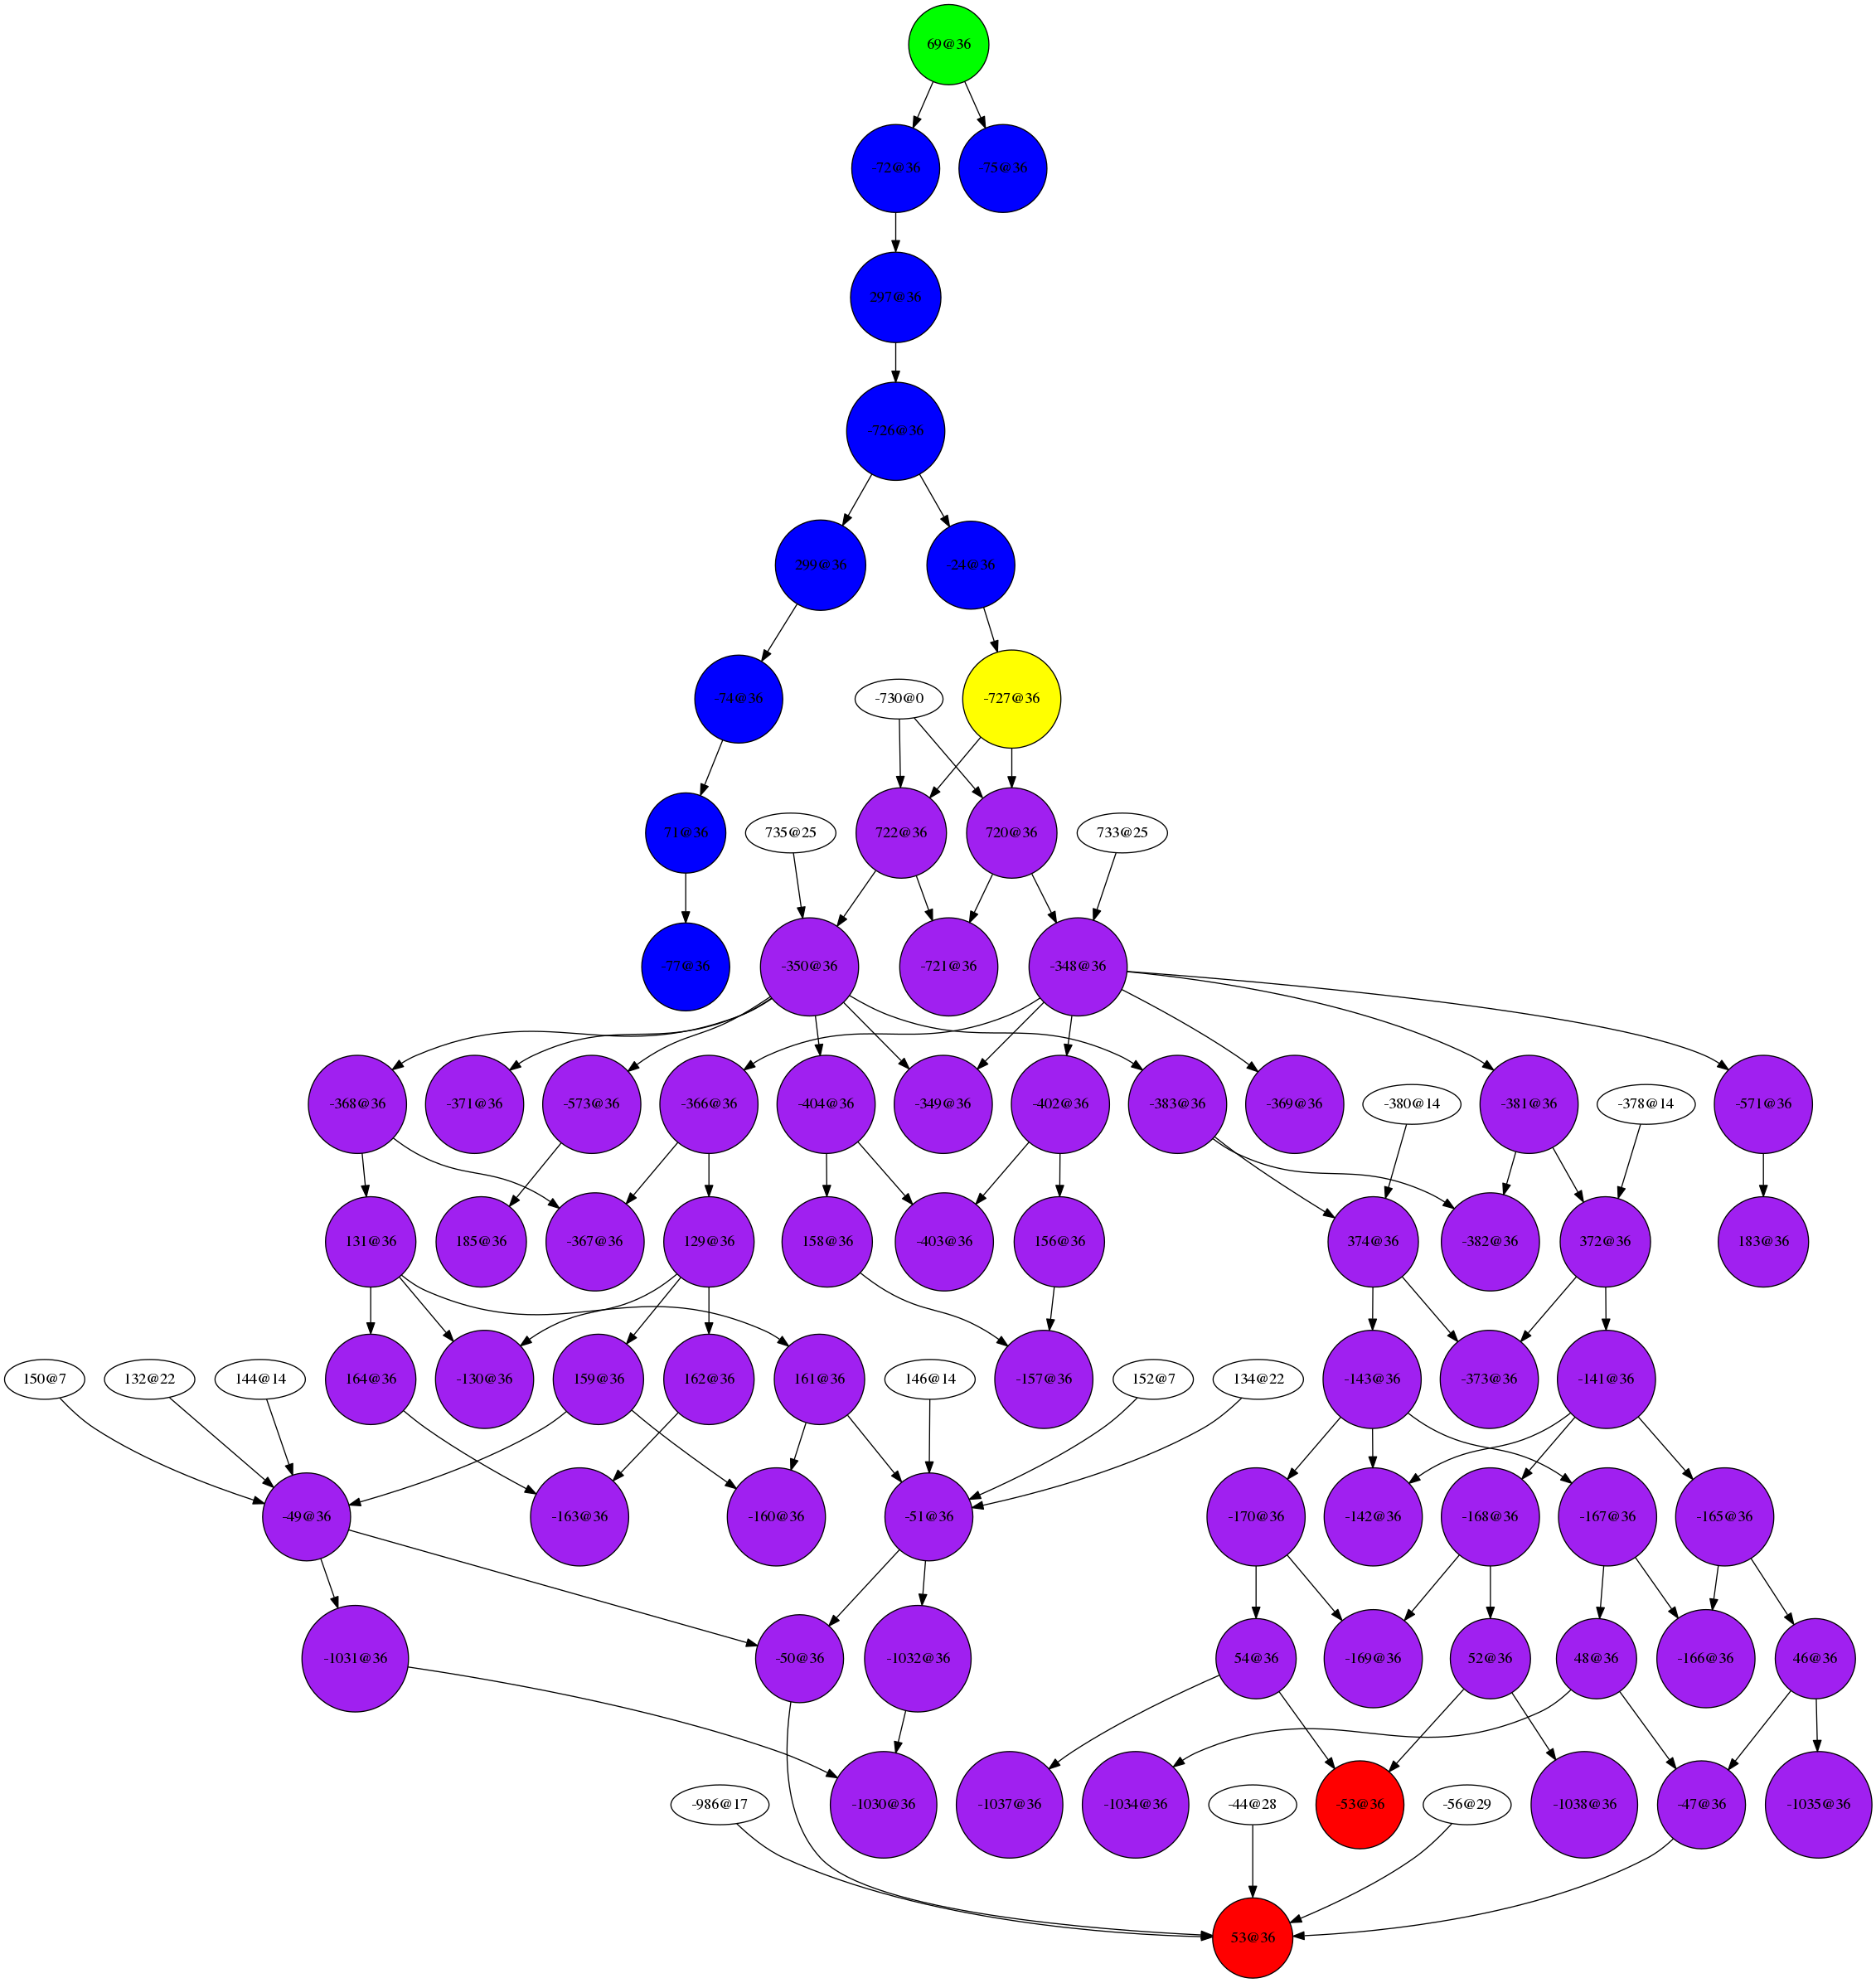
\includegraphics[scale=0.15]{graphe.png}
            \end{center}
        \end{frame}

    \section{Résultats}
        \begin{frame}{Résultats}{}
            \begin{center}
                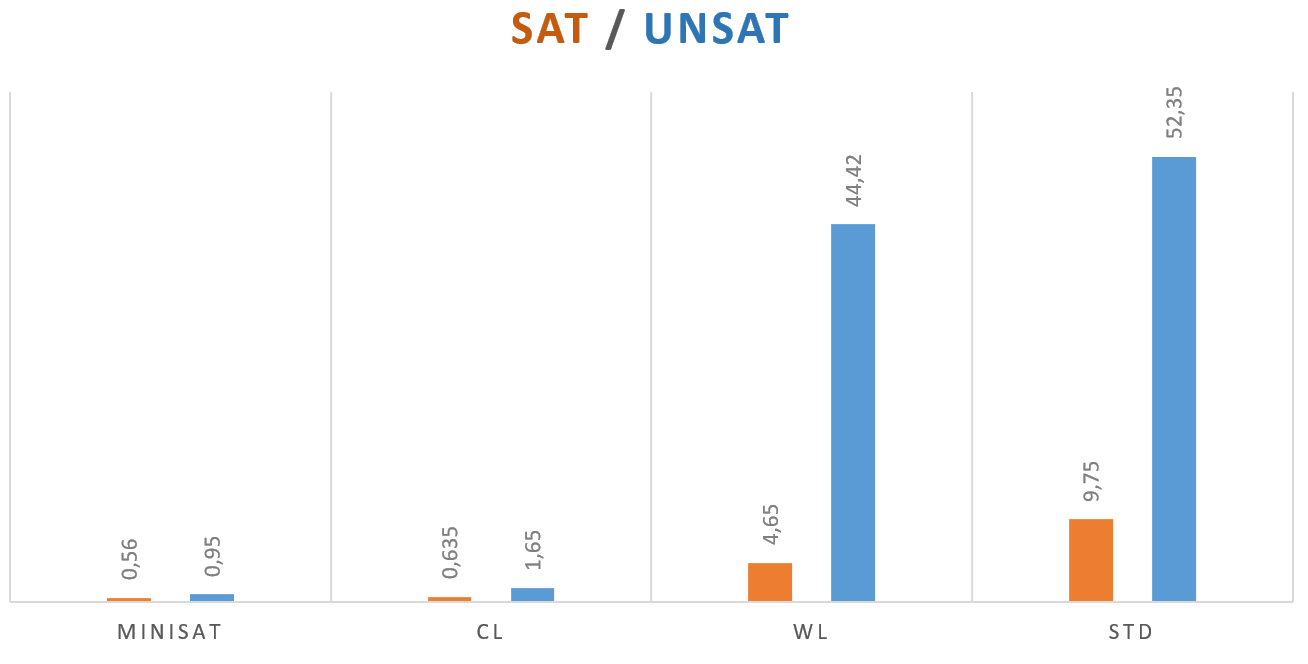
\includegraphics[scale=0.25]{time.png}
            \end{center}
        \end{frame}       

\end{document}
